\documentclass[12pt, 
hyperref={colorlinks=true, linkcolor=BlueViolet, urlcolor=BlueViolet},dvipsnames]{beamer}
\usetheme{default} 

\setbeamertemplate{navigation symbols}{} %gets rid of navigation symbols
\setbeamertemplate{footline}{} %gets rid of bottom navigation bars
\setbeamertemplate{footline}[page number]{} %use this for page numbers

\setbeamertemplate{footline}{%
  \raisebox{5pt}{\makebox[\paperwidth]{\hfill\makebox[10pt]{\scriptsize\insertframenumber~~}}}}

\setbeamertemplate{itemize items}[circle] %round bullet points
\setlength\parskip{10pt} % white space between paragraphs

\usepackage{wrapfig}
\usepackage{subfig}
\usepackage{setspace}
\usepackage{enumerate}
\usepackage{graphicx}
\usepackage{amsmath}
\usepackage{amsfonts}
\usepackage{amssymb}
\usepackage{amsthm}
\usepackage[UKenglish]{isodate}
\usepackage{verbatim}
\usepackage{xcolor}
\cleanlookdateon

% new amber color
\definecolor{amber}{rgb}{1.0, 0.75, 0.0}


% the preamble
\title{Lecture 9: Cluster computing}
\author{Brian Williamson}
\institute{BIOST 561: Computational Skills For Biostatistics I}
\date{29 May 2019}

% Start the document
\begin{document}
% The title page
\begin{frame}
\titlepage
\end{frame}

% motivation
\section{Introduction}
\begin{frame}
\frametitle{Motivation}
We are often interested in \textcolor{cyan}{large-scale} computing: \vspace{-0.3cm} \pause
\begin{itemize}
\item simulation studies (e.g., lecture 4) \pause
\item intensive data analyses (e.g., \href{https://www.nejm.org/doi/full/10.1056/nejmoa1702747}{air pollution and mortality}) \pause
\end{itemize}

In Lecture 8, you learned how to compute without \texttt{R}. 

Today, you'll learn how to transfer those skills to computing on a \textcolor{ForestGreen}{cluster}.

\end{frame}

\begin{frame}
\frametitle{Examples from my research}
\textcolor{cyan}{Large-scale} simulation studies: \vspace{-0.3cm} \pause
\begin{itemize}
\item proof-of-concept examples \pause
\item showcase \textcolor{ForestGreen}{operating characteristics} of proposed method
\end{itemize} \pause

\begin{center}
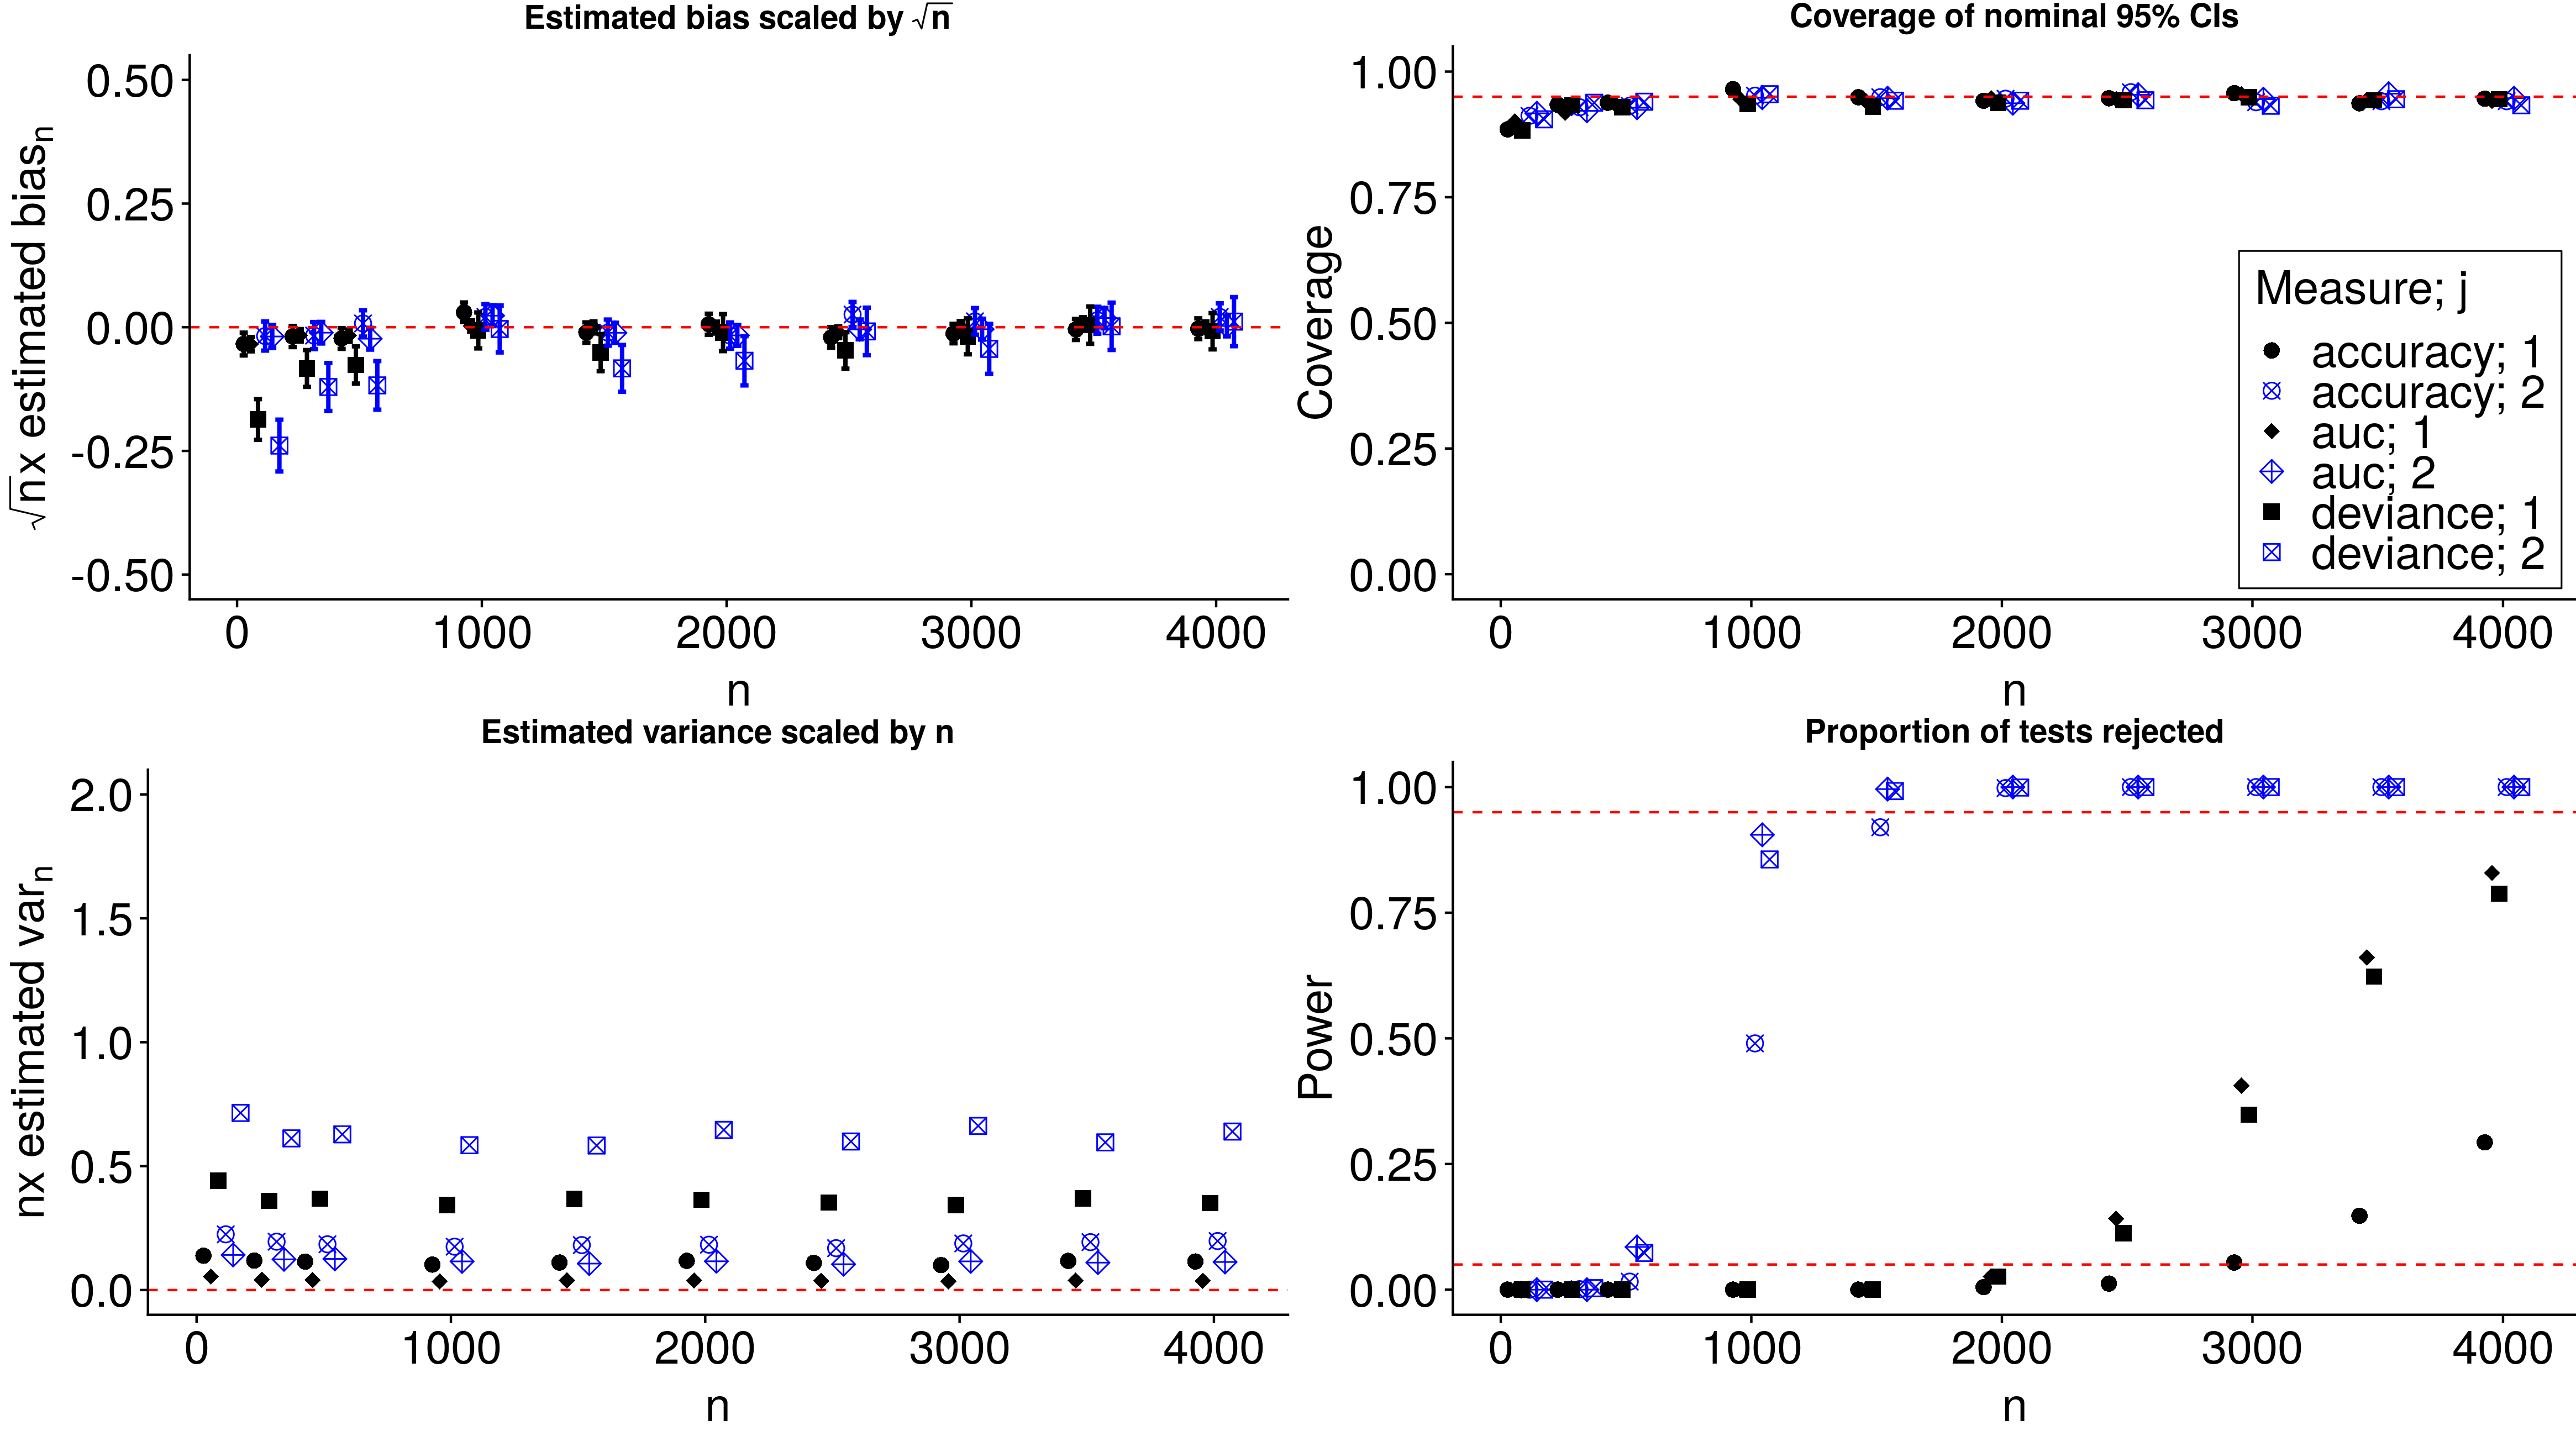
\includegraphics[width = 1\textwidth]{plots/bivariate_loss_performance_deviance_accuracy_auc.png}
\end{center}
\end{frame}

\begin{frame}
\frametitle{Examples from my research}
\textcolor{BurntOrange}{Data analysis}: \vspace{-0.3cm} \pause
\begin{itemize}
\item fit a time-consuming estimator \pause
\item cross-validation? \pause
\item memory-intensive computations? \pause
\end{itemize}

\begin{center}
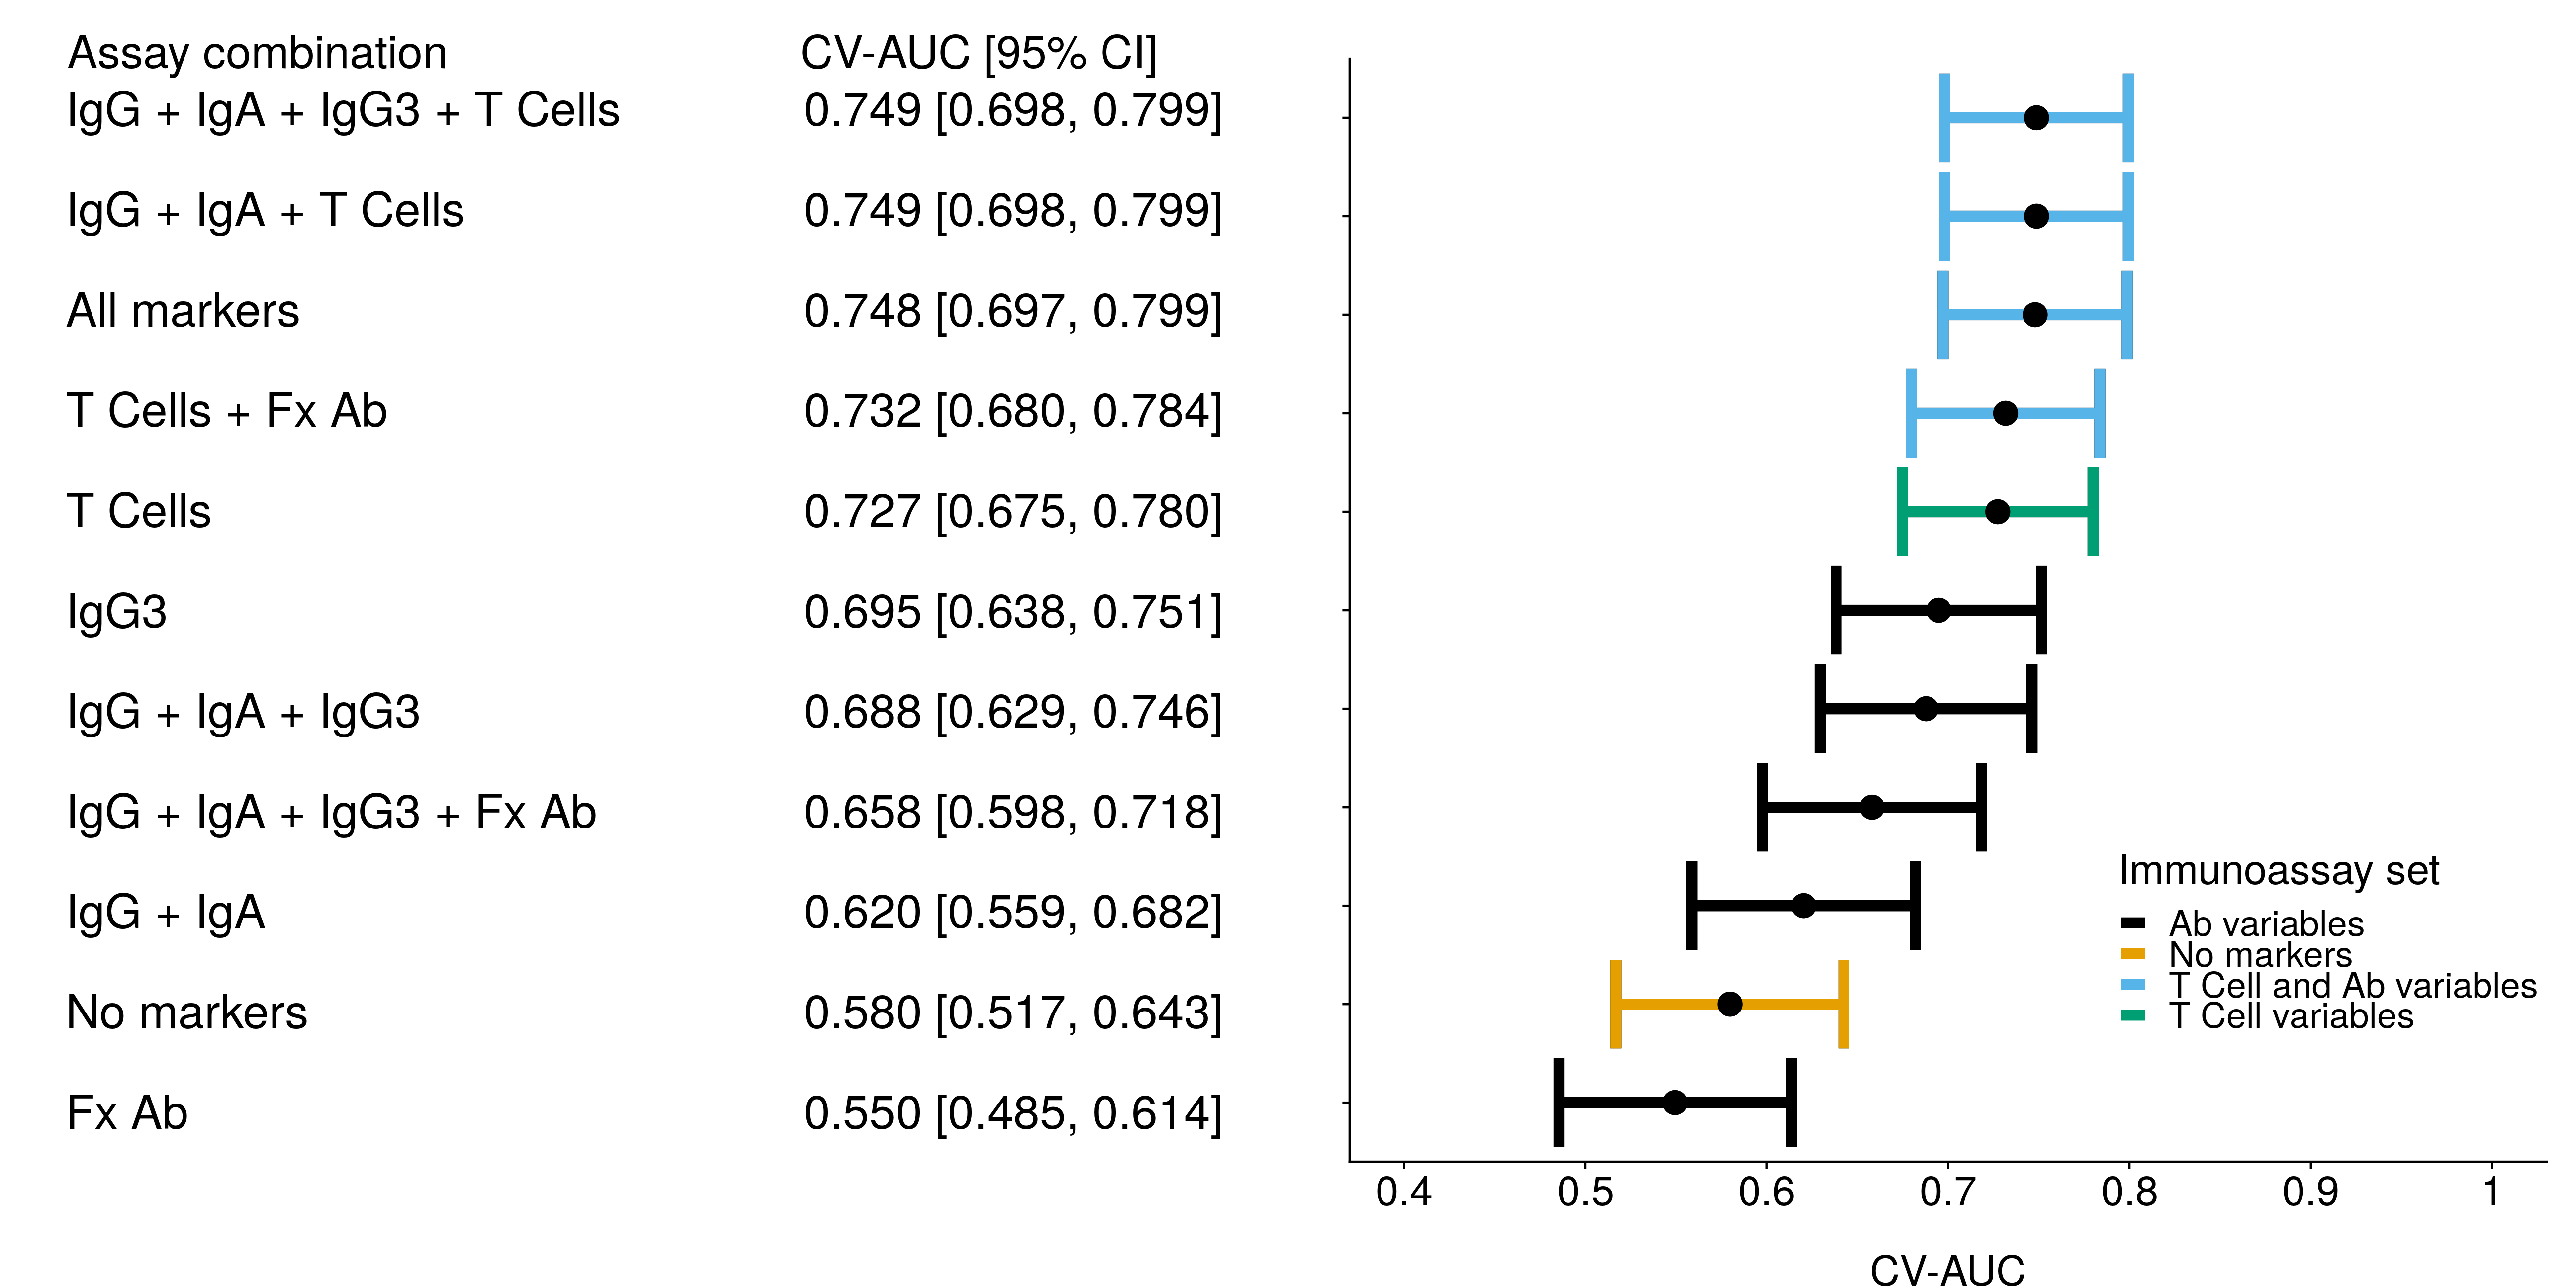
\includegraphics[width = 1\textwidth]{plots/cv_auc_forest_plot_sl.png}
\end{center}
\end{frame}

\begin{frame}
\frametitle{The problem}
How do I run\vspace{-0.3cm} \pause
\begin{itemize}
\item \textcolor{blue}{many} \pause
\item potentially \textcolor{red}{time-consuming} \pause
\item or \textcolor{red}{memory-intensive} \pause
\end{itemize}
analyses without \pause keeping an R session open (\textcolor{red}{for the duration!}) \pause \textcolor{red}{on my personal machine}?
\end{frame}

\begin{frame}
\frametitle{The solution}
Cluster computers provide a solution! \pause

Cluster computers: \vspace{-0.3cm} \pause
\begin{itemize}
\item allow you to \textcolor{blue}{submit multiple \textbf{jobs}${}^*$ at once} \pause
\item can \textcolor{blue}{schedule jobs for you} \pause
\item are \textcolor{blue}{optimized} for high-performance computing (HPC) \pause
\end{itemize}

{\small ${}^*$: we will discuss this further!}
\end{frame}

\begin{frame}
\frametitle{Running example: robust standard errors (SEs)}

Consider a sample of $n$ observations generated iid according to
\begin{align*}
X \sim & \ N(0, 1), \\
u \sim & \ N(0, 1), \text{ independent of $X$}; \\
Y \mid X, u =& \ \beta_0 + \beta_1 X + \epsilon, \text{ where } \\
\epsilon =& \ \lvert X \rvert u.
\end{align*}

Questions: can we use \vspace{-0.3cm}
\begin{enumerate}
\item linear regression to estimate $\beta_1$? \pause \textcolor{blue}{Yes!} \pause
\item model-based standard errors to estimate $sd(\beta_1)$? \pause \textcolor{red}{No!} \pause
\item robust standard errors to estimate $sd(\beta_1)$? \pause \textcolor{blue}{Yes!}
\end{enumerate}
\end{frame}

\begin{frame}
\frametitle{Running example: robust SEs}
Goals: \vspace{-0.3cm}  \pause
\begin{itemize}
\item compare model-based to robust SEs \pause
\item do this without using our own computers \pause
\end{itemize}

We will use the cluster to do this!
\end{frame}

% section 1: coding in a cluster-friendly way
\section{Coding for the cluster}
\begin{frame}
\frametitle{}
\begin{center}
{\large \textbf{Part I: coding for the cluster}}
\end{center}
\end{frame}

\begin{frame}
\frametitle{Coding for the cluster}
Before moving to the cluster, we need to code differently: \vspace{-0.3cm} \pause
\begin{itemize}
\item 
\end{itemize}
\end{frame}

\begin{frame}
\frametitle{Coding for the cluster: modular code}

\end{frame}

\begin{frame}
\frametitle{Coding for the cluster: setting the seed}

\end{frame}

\begin{frame}
\frametitle{Coding for the cluster: saving output}

\end{frame}

\begin{frame}
\frametitle{Coding for the cluster: debugging}

\end{frame}


\begin{frame}
\frametitle{Coding for the cluster: compiling output}

\end{frame}

% section 2: using the cluster
\section{Using the cluster}
\begin{frame}
\frametitle{}
\begin{center}
{\large \textbf{Part II: using the cluster}}
\end{center}
\end{frame}

\begin{frame}
\frametitle{Using the cluster}
Department resources for HPC${}^*$: \vspace{-0.3cm} \pause
\begin{itemize}
\item \texttt{cox}: 12-core computer \pause (\textcolor{red}{not a cluster}) \pause
\item \texttt{bayes}: compute cluster
\end{itemize}

A cluster consists of: \vspace{-0.3cm} \pause
\begin{itemize}
\item a head node \pause (where you are) \pause
\item compute nodes \pause (where your code gets run) \pause
\item submission system \pause (how your code gets run) \pause
\end{itemize}

{\small ${}^*$other groups have similar resources, e.g., \vspace{-0.3cm}
\begin{itemize}
\item \href{https://itconnect.uw.edu/service/shared-scalable-compute-cluster-for-research-hyak/}{\texttt{hyak}} (managed by UW-IT)
\item \texttt{pearson} (statistical genetics group only)
\item \texttt{gizmo} (Fred Hutchinson Cancer Research Center only)
\item Microsoft Azure, Amazon Web Services (AWS)
\end{itemize}
}
\end{frame}

\begin{frame}
\frametitle{Using the cluster}
\begin{center}
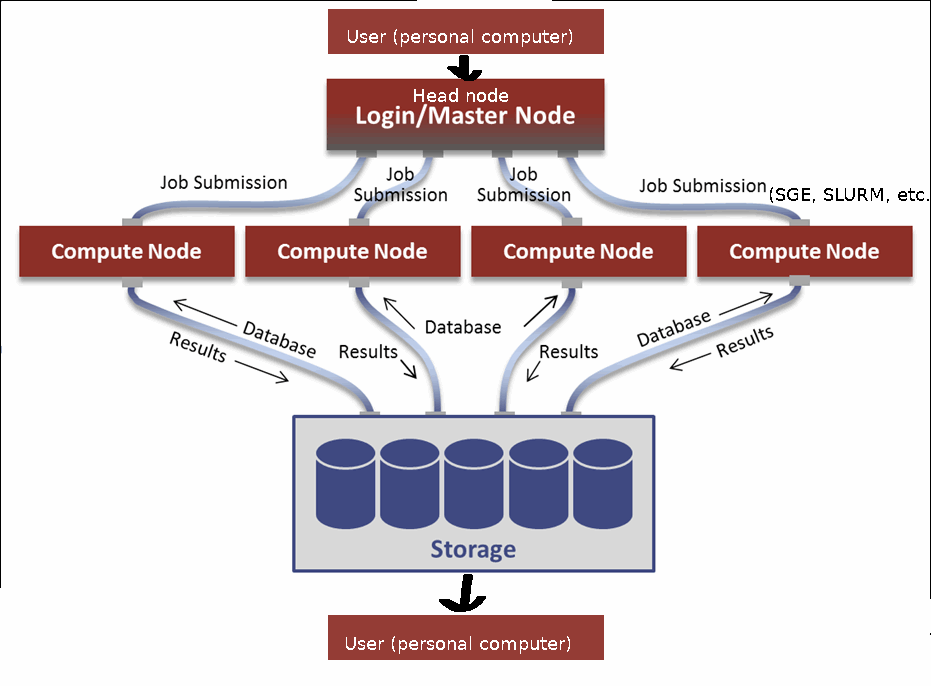
\includegraphics[width = 1\textwidth]{plots/hpc_system.png}
\end{center}
\end{frame}

\begin{frame}
\frametitle{Using the cluster: \texttt{bayes}}
More specifically, \texttt{bayes} \vspace{-0.3cm} \pause
\begin{itemize}
\item has \textcolor{cyan}{4 department-wide} compute nodes, each with \textcolor{blue}{12 cores} \pause
\item uses Sun Grid Engine (\href{https://en.wikipedia.org/wiki/Oracle_Grid_Engine}{SGE}) for submissions \pause
\end{itemize}

Since this is a shared resource, being \textcolor{blue}{nice} is important: \vspace{-0.3cm} \pause
\begin{itemize}
\item don't run simulations on the head node \pause
\item don't flood the cluster \pause
\end{itemize}

We'll practice good habits for being nice as we go along.
\end{frame}



\begin{frame}
\frametitle{Using the cluster: logging in (Windows, incl.~\texttt{box})}
\begin{enumerate}
\item Open TeraTerm [or your favorite secure shell (SSH) client]
\item Enter the address of your favorite cluster, e.g., \texttt{bayes.biostat.washington.edu}
\item Make sure that the ``New connection'' window is filled out as in the figure, except for ``Host'' (screenshot from \texttt{box})
\item Click \texttt{OK}, enter your UW BIOST username and password when prompted (user and pass you use for \texttt{box}) 
\end{enumerate}
\centering
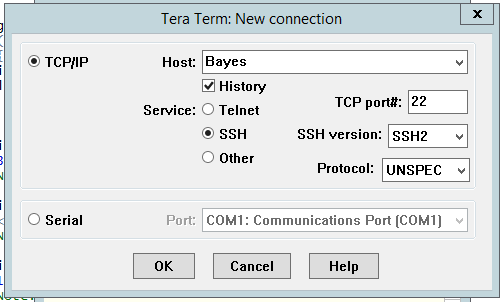
\includegraphics[width = .45\textwidth]{plots/tera_term_example.png}
\end{frame}

\begin{frame}
\frametitle{Using the cluster: logging in (Mac/Linux)}
\begin{enumerate}
\item Open a Terminal window
\item[]
\item Type \texttt{ssh mynetid@cluster.washington.edu}
\begin{itemize}
\item replace \texttt{mynetid} with Your UW NetID, and 
\item replace \texttt{cluster} with Your cluster, e.g., \texttt{bayes}
\end{itemize} 
\item[]
\item Enter password (same password as \texttt{box}) when prompted (the field will remain blank but your password will be received)
\end{enumerate}

\end{frame}

\begin{frame}
\frametitle{Using the cluster: logging in}
Your turn!
\begin{enumerate}
\item Log into the cluster
\item What is the name of the directory that you are when you log in?
\item Create a directory called \texttt{robust\_ses} in your \texttt{home} directory
\item Create a directory called \texttt{robust\_ses} on \textbf{your} computer, under \texttt{biost561/lecture9}
\end{enumerate}
\end{frame}

\begin{frame}
\frametitle{Using the cluster: moving around}
The cluster runs on Linux: in particular, the tools you learned in lecture 8, including \vspace{-0.3cm} \pause
\begin{itemize}
\item navigation, \pause
\item vim, \pause
\item commands, \pause and
\item shell scripts
\end{itemize}
are all used \textcolor{blue}{in exactly the same way}!
\end{frame}

\begin{frame}
\frametitle{Using the cluster: jobs}
The basic unit of cluster computing is a \textcolor{cyan}{job}. \pause

Jobs: \vspace{-0.3cm} \pause
\begin{itemize}
\item perform a specified task \pause
\item can be submitted to the cluster compute nodes \pause
\end{itemize}

Example job: 
\end{frame}

\begin{frame}
\frametitle{Using the cluster: jobs}
\begin{center}
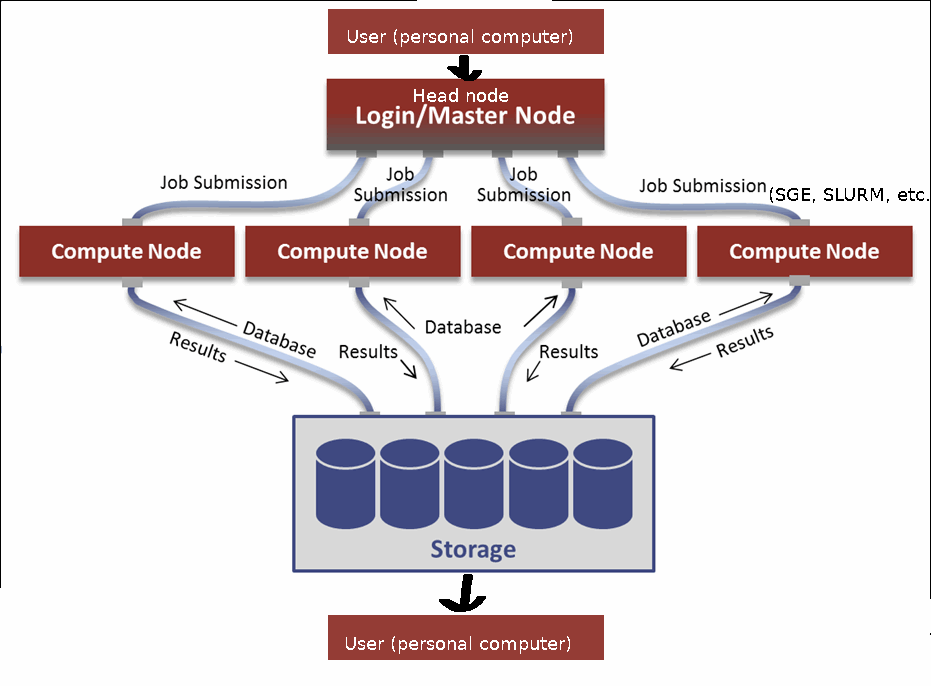
\includegraphics[width = 1\textwidth]{plots/hpc_system.png}
\end{center}
\end{frame}

\begin{frame}
\frametitle{Using the cluster: submitting jobs}
Workhorse command on SGE: \href{http://gridscheduler.sourceforge.net/htmlman/htmlman1/qsub.html}{qsub}

Many options, including: \vspace{-0.3cm} \pause
\begin{itemize}
\item 
\end{itemize}

Options are specified with a single \texttt{-}, as you saw in Lecture 8.
\end{frame}

\begin{frame}
\frametitle{Using the cluster: checking jobs}

\end{frame}

\begin{frame}
\frametitle{Using the cluster: other helpful SGE commands}
\end{frame}

% section 3: appendix, other useful commands
\section*{Appendix: other useful cluster things}
\begin{frame}
\frametitle{}
\begin{center}
{\large \textbf{Appendix: other useful cluster things}}
\end{center}
\end{frame}
\begin{frame}
\frametitle{Useful things: Windows file compatability}
\end{frame}
\end{document}
